\documentclass{article}
%\usepackage{apacite}
\usepackage{graphicx}
\usepackage{hyperref}

\title{Text-Mining the arXiv with LLMs}
\author{Luis Berlioz\\
    Universidad Nacional Autónoma de Honduras}


\begin{document}
\begin{abstract}
    We introduce ArGoT, a data set of mathematical terms extracted from 
the articles hosted on the arXiv website. 
A term is any mathematical concept defined in an article.
Using labels in the article's source code and examples from other
popular math websites, we mine all the terms in the
arXiv data and compile a comprehensive vocabulary of mathematical terms.
Each term can be then organized in a dependency graph by using
the term's definitions and the arXiv's metadata.
Using both hyperbolic and standard word embeddings, we demonstrate how 
this structure is reflected in the text's vector representation and
how they capture relations of entailment in mathematical concepts. This
data set is part of an ongoing effort to align natural mathematical
text with existing Interactive Theorem Prover  Libraries (ITPs) of
formally verified statements.
%% Include Formal abstracts project

\end{abstract}
\section{Introduction}
%In previous works \cite{Deyan1, glossary, scss}, 
%This work relies on the methodology in \cite{Deyan1, glossary, scss}, to generate the training sets that are used in this 

This work describes the process of finetuning large language models (LLMs) to generate a complete glossary of mathematics from the arXiv website.  It starts with the finetuning of pretrained LLMs for two different tasks. The first is the classification task, in which a sequence classifier is trained on examples of mathematical definitions and non-definitions. This binary classifier is run on the paragraphs from the mathematics articles stored in the arXiv website. The classification task is followed by the NER task (also known as chunking) in which the terms being defined (definienda) are identified. This task is performed using a token classifier and it is run on all the definitions from the previous step. The resulting dataset of definitions and terms can be browsed here: \url{https://efedequis.xyz/argot/}

In the classification task, a binary sequence classifier is trained on a dataset that contains labeled paragraphs. The labels are set according to whether each paragraph is a definition or not. This dataset is obtained using the methodology in \cite{Deyan1}, in which the \LaTeX{} source of the articles is parsed in search of the \verb|\begin{definition}...\end{definition}| macro. The parsing of the documents was done with LaTeXML (\url{https://math.nist.gov/~BMiller/LaTeXML/}), which is a package designed to convert \TeX{} source code into documents in XML format. 
The negative examples are generated by negative sampling, i.e.\ randomly selecting paragraphs from articles and labeling them as non-definitions. The amount of both categories is set to be roughly the same to produce a balanced dataset. 

Similarly for the NER task, a training set was automatically produced using the methodoly in \cite{scss}. This methodology uses the the content of freely available websites like Planetmath \url{https://planetmath.org/}, The Stacks project \url{https://stacks.math.columbia.edu/} and Wikipedia. The training data for this task requires each word in a definition to be labeled as whether or not it is part of the term being defined. This annotation is done automatically by exploiting the standard format of these websites. Many websites that introduce a mathematical or scientic term include a Definition section, the term being defined is usually the title of the website. The definition is annotated by searching for the title in the text of the definition. Figure~\ref{stacks} shows an example of this process from the Stacks project.

\begin{figure}\label{stacks}
    \centering
    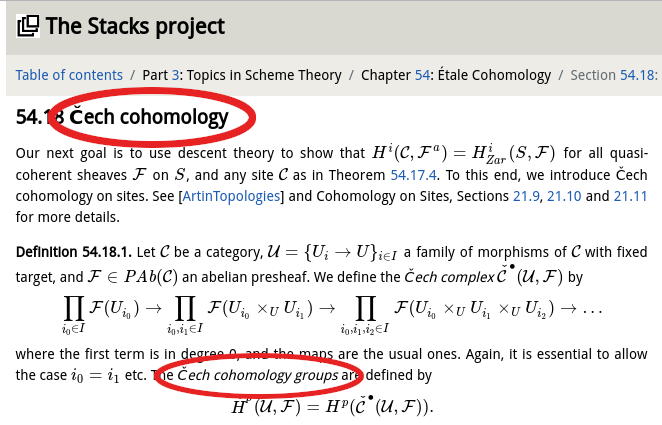
\includegraphics[width=0.7\textwidth]{Images/stacks_defs.png}
    \caption{Example of a definition being annotated by searching the name of the article inside the definition section of the website.}
\end{figure}

Several common LLMs can be finetuned to classify short texts. This process is generally called 

The methodology used to produce a training set of labeled definitions appears in \cite{Deyan1, glossary}. It consists of parsing the \LaTeX{} source of the mathematical articles in search of 

To 


\section{Training}
both classification task and NER
Scatter plot of training sessions.

\section{Inference}
Just describe the parallelization and time spent

\section{Conclusions and Future Work}

\bibliographystyle{apalike}
\bibliography{article}
\end{document}
